\subsubsection{Interlayer service}

This component is responsible of the communication that is performed among
different layers, namely the one which it belongs (the \textbf{middleware}) and
another one who uses the middleware layer, that is the \textbf{application}
layer.

We show in figure \ref{fig:mw-interlayer} the architecture of this service and
then we will show in detail each module that composes this component.

\begin{figure}[H]
  \centering
  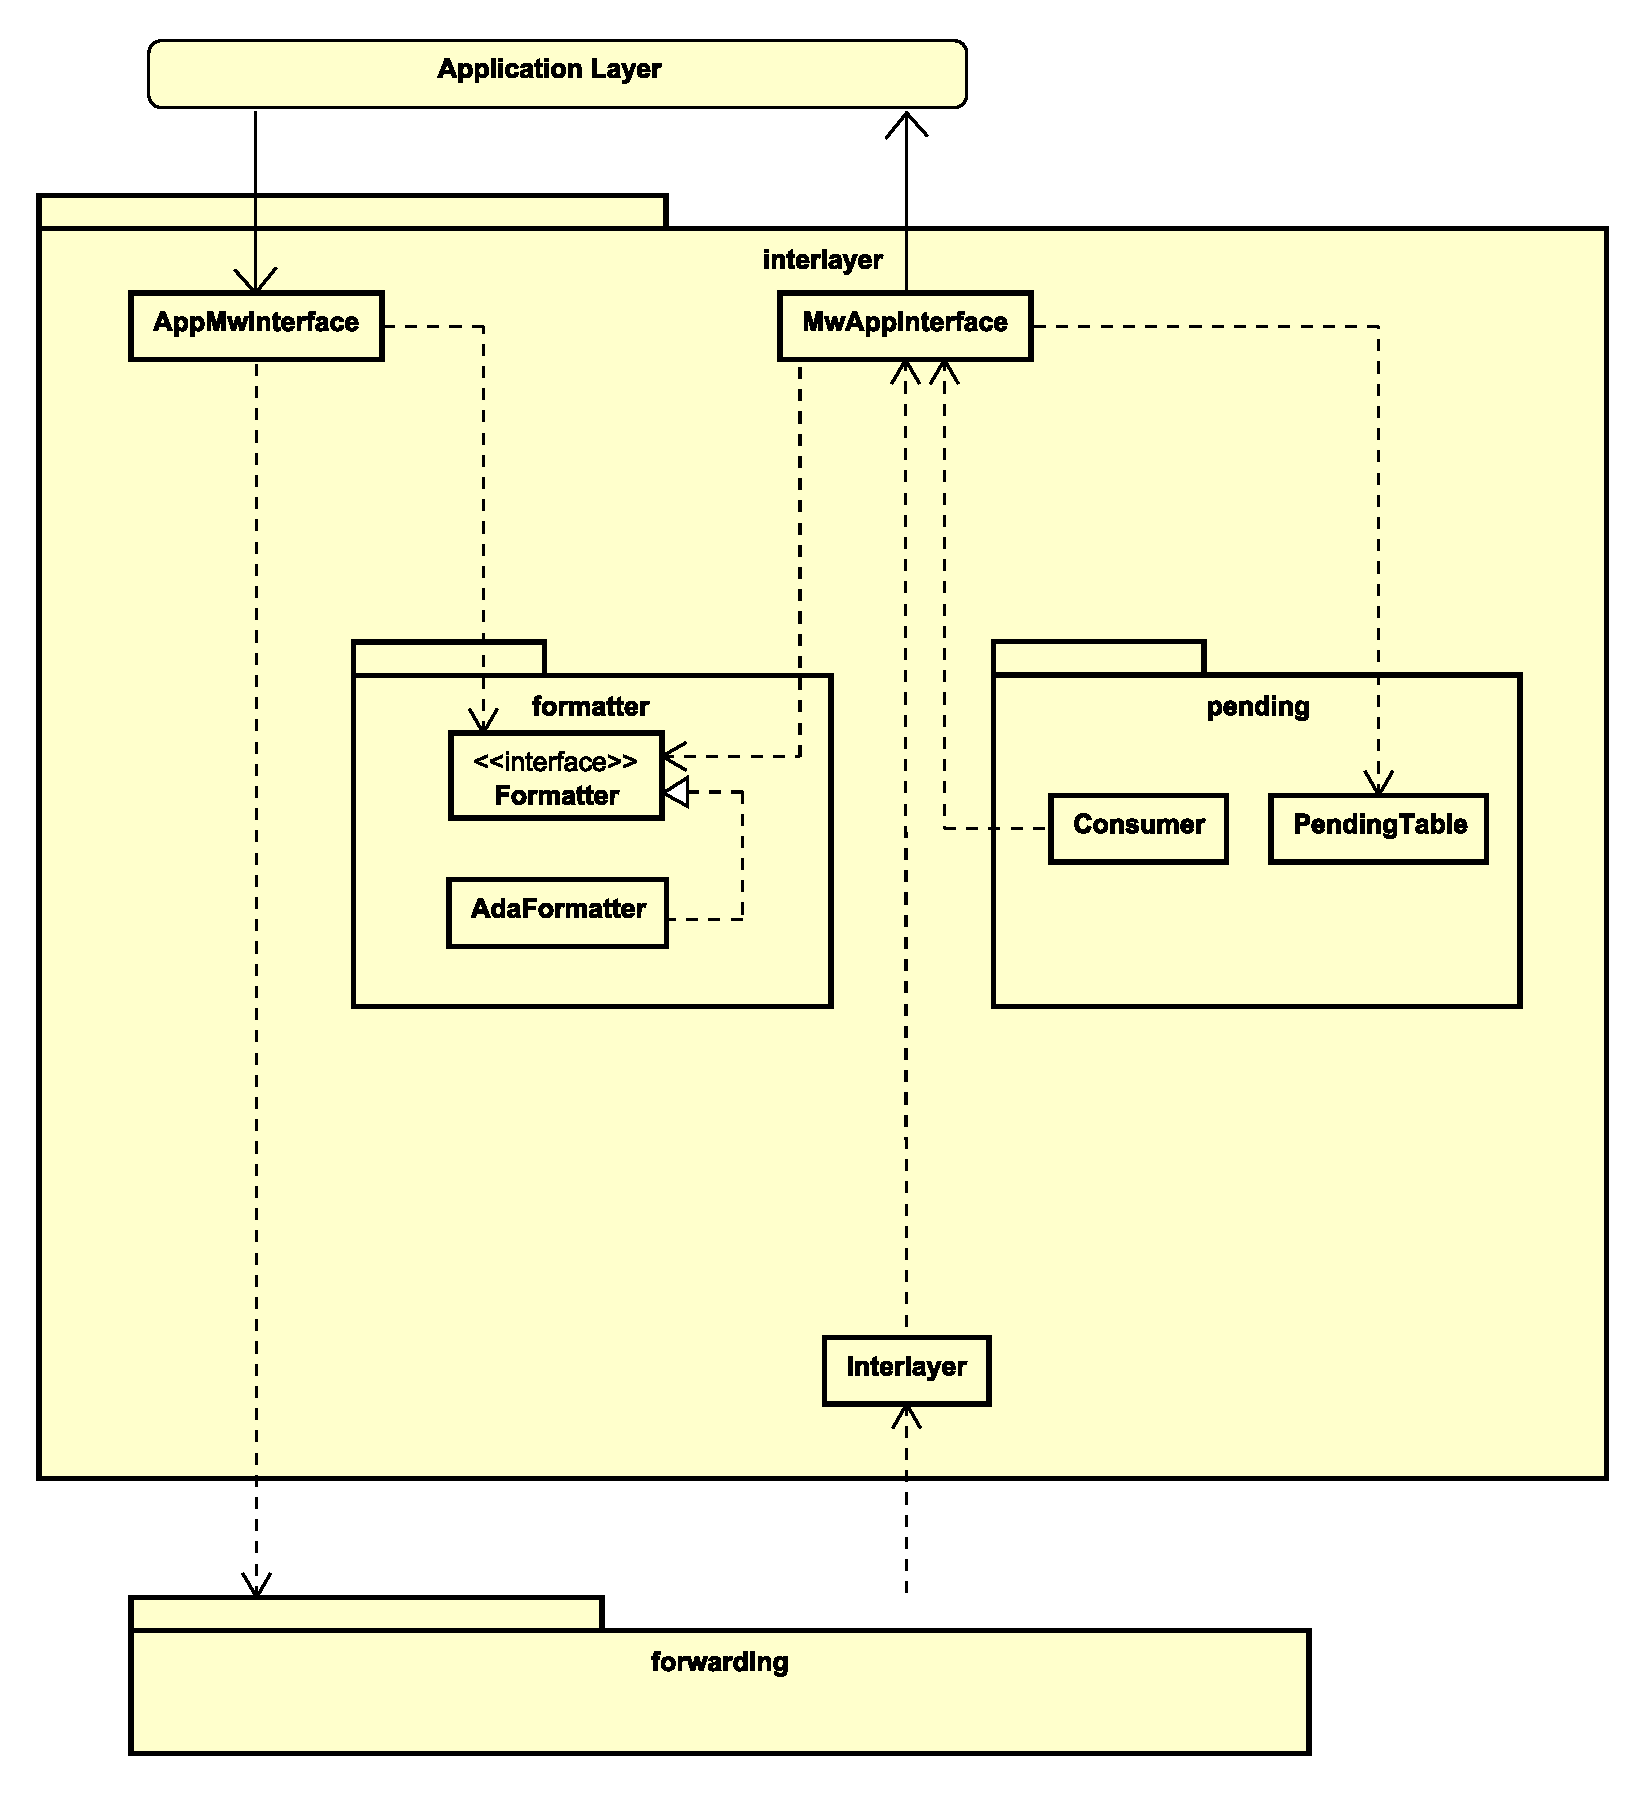
\includegraphics[width=\columnwidth]{images/solution/mw/interlayer.eps}
  \caption{Middleware's Interlayer service}
  \label{fig:mw-interlayer}
\end{figure}

\subsubsubsection{interlayer.Interlayer}

\begin{figure}[H]
  \centering
  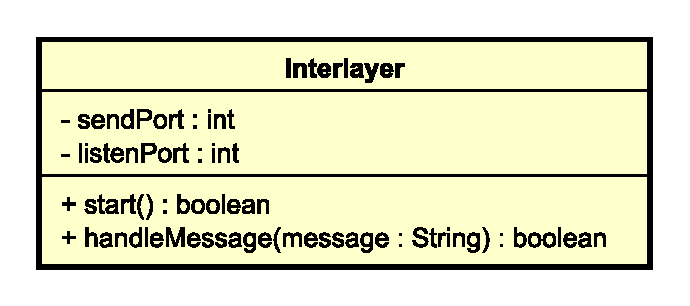
\includegraphics[width=.5\columnwidth]{images/solution/mw/int/inter.eps}
  \caption{interlayer.Interlayer}
  \label{fig:mw-interlayer-interlayer}
\end{figure}
    % TODO: check this out: will Message actually be a String?

\FloatBarrier
\begin{itemize}
  \item \textbf{Description} \\
    This module is the Fa\c cade of the Interlayer service. It is responsible
    to boot neatly and supervise all processes in Interlayer.
  \item \textbf{Attributes}
    \begin{itemize}
      \item \texttt{- sendPort: Int} \\
    TCP port messages will be directed to.
      \item \texttt{- listenPort: Int} \\
    TCP port messages will be received from.
    \end{itemize}
  \item \textbf{Operations}
  \begin{itemize}
    \item \texttt{+ start()} \\
    % TODO: check this out: will Message actually be a String?
    Starts the Interlayer service.
    \item \texttt{+ handleMessage(message: String)} \\
    % TODO: check this out: will Message actually be a String?
    Handles the reception of a message by ensuring it reaches the application
    layer.
  \end{itemize}
\end{itemize}

\subsubsubsection{interlayer.MwAppInterface}

\begin{figure}[H]
  \centering
  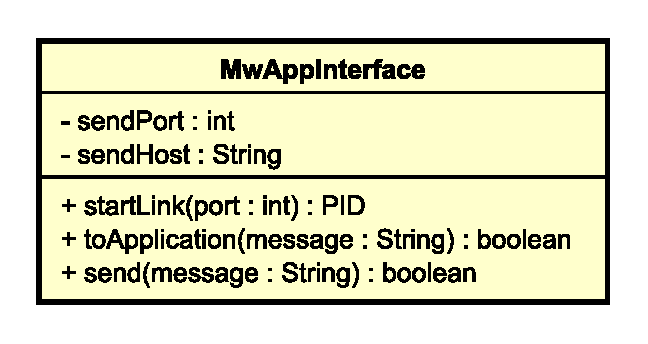
\includegraphics[width=.5\columnwidth]{images/solution/mw/int/mwapp.eps}
  \caption{interlayer.MwAppInterface}
  \label{fig:mw-interlayer-mwappinterface}
\end{figure}
    % TODO: check this out: will Message actually be a String?

\FloatBarrier
\begin{itemize}
  \item \textbf{Description} \\
    Process that is responsible to deliver messages to the application layer.
  \item \textbf{Attributes}
    \begin{itemize}
      \item \texttt{- sendPort: Int} \\
    TCP port messages will be directed to.
      \item \texttt{- sendHost: String} \\
    Address messages will be directed to.
    \end{itemize}
  \item \textbf{Operations}
  \begin{itemize}
    \item \texttt{+ startLink(port: Int)} \\
    Starts the process and set \texttt{sendPort} to the value \texttt{port}.
    \item \texttt{+ toApplication(message: String)} \\
    % TODO: check this out: will Message actually be a String?
    Sends a message to the application with reliable delivery.
    \item \texttt{+ send(message: String)} \\
    % TODO: check this out: will Message actually be a String?
    Sends a message to the application with unreliable delivery.
  \end{itemize}
\end{itemize}

\subsubsubsection{interlayer.AppMwInterface}

\begin{figure}[H]
  \centering
  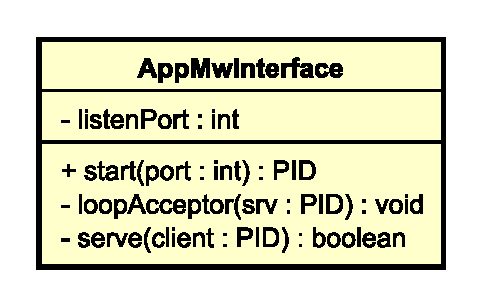
\includegraphics[width=.4\columnwidth]{images/solution/mw/int/appmw.eps}
  \caption{interlayer.AppMwInterface}
  \label{fig:mw-interlayer-appmwinterface}
\end{figure}

\FloatBarrier
\begin{itemize}
  \item \textbf{Description} \\
    Process that is responsible to receive messages from the application layer.
  \item \textbf{Attributes}
    \begin{itemize}
      \item \texttt{- listenPort: Int} \\
    TCP port messages will be received from.
    \end{itemize}
  \item \textbf{Operations}
  \begin{itemize}
    \item \texttt{+ start(port: Int)} \\
    Starts a server, setting \texttt{listenPort} to the value \texttt{port}.
    \item \texttt{- loopAcceptor(srv: PID)} \\
    Loops accepting requests as the server \texttt{srv}.
    \item \texttt{- serve(client: PID)} \\
    Handles the stream coming from the TCP connection of \texttt{client} by
    forwarding data towards to the Forwarding service.
  \end{itemize}
\end{itemize}

\subsubsubsection{interlayer.formatter.Formatter}

\begin{figure}[H]
  \centering
  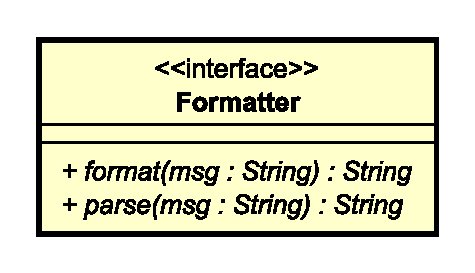
\includegraphics[width=.4\columnwidth]{images/solution/mw/int/form.eps}
  \caption{interlayer.formatter.Formatter}
  \label{fig:mw-interlayer-formatter-formatter}
\end{figure}
    % TODO: check this out: will Message actually be a String?

\FloatBarrier
\begin{itemize}
  \item \textbf{Description} \\
    Interface for modules that translates messages to Elixir format from and
    to a (possibly) different one.
  \item \textbf{Operations}
  \begin{itemize}
    \item \texttt{+ format(msg: String)} \\
    Translates \texttt{msg} to the target format.
    % TODO: check this out: will Message actually be a String?
    \item \texttt{+ parse(msg: String)} \\
    Translates \texttt{msg} from the target format.
  \end{itemize}
\end{itemize}

\subsubsubsection{interlayer.formatter.AdaFormatter}

\begin{figure}[H]
  \centering
  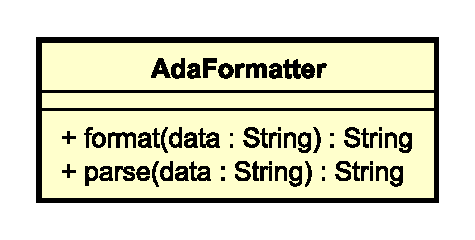
\includegraphics[width=.4\columnwidth]{images/solution/mw/int/adaform.eps}
  \caption{interlayer.formatter.AdaFormatter}
  \label{fig:mw-interlayer-formatter-adaformatter}
\end{figure}
    % TODO: check this out: will Message actually be a String?

\FloatBarrier
\begin{itemize}
  \item \textbf{Description} \\
    Module that implements the \texttt{interlayer.formatter.Formatter}
    interface for messages coming from an Ada application.
  \item \textbf{Attributes}
  \item \textbf{Operations}
  \begin{itemize}
    \item \texttt{+ format(data: String)} \\
    Format a message so that it can be received from an Ada application.
    % TODO: check this out: will Message actually be a String?
    \item \texttt{+ parse(data: String)} \\
    Parse a message that arrives from an Ada application.
  \end{itemize}
\end{itemize}

\subsubsubsection{interlayer.pending.PendingTable}

\begin{figure}[H]
  \centering
  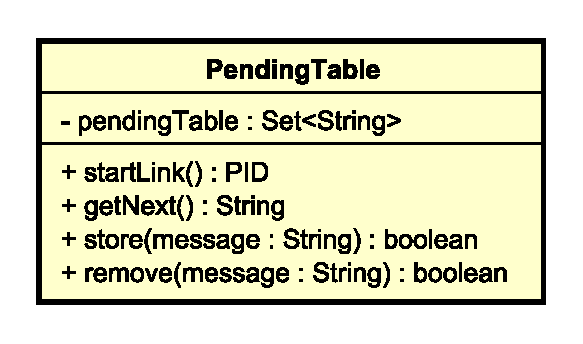
\includegraphics[width=.5\columnwidth]{images/solution/mw/int/pendtbl.eps}
  \caption{interlayer.pending.PendingTable}
  \label{fig:mw-interlayer-pending-pendingtable}
\end{figure}
    % TODO: check this out: will Message actually be a String?

\FloatBarrier
\begin{itemize}
  \item \textbf{Description} \\
    Process that keeps track of the messages that have not been sent yet to
    the application layer.
  \item \textbf{Attributes}
    \begin{itemize}
      \item \texttt{- pendingTable: Set<String>} \\
    Data structure in which pending messages are stored.
    % TODO: check this out: will Message actually be a String?
    \end{itemize}
  \item \textbf{Operations}
  \begin{itemize}
    \item \texttt{+ startLink()} \\
    Starts PendingTable process and retrieves pending messages from last
    execution (if there are some). \\
    Also starts at least one \texttt{interlayer.pending.Consumer}.
    \item \texttt{+ getNext()} \\
    If there are some pending messages, returns the first of them that has to
    be sent.
    \item \texttt{+ store(message: String)} \\
    Stores a message in the pending table.
    % TODO: check this out: will Message actually be a String?
    \item \texttt{+ remove(message: String)} \\
    Removes a message from the pending table.
    % TODO: check this out: will Message actually be a String?
  \end{itemize}
\end{itemize}

\subsubsubsection{interlayer.pending.Consumer}

\begin{figure}[H]
  \centering
  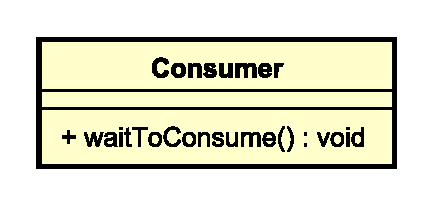
\includegraphics[width=.4\columnwidth]{images/solution/mw/int/cons.eps}
  \caption{interlayer.pending.Consumer}
  \label{fig:mw-interlayer-pending-consumer}
\end{figure}
    % TODO: check this out: will Message actually be a String?

\FloatBarrier
\begin{itemize}
  \item \textbf{Description} \\
    Daemon worker that sequentially takes message from the pending table and
    tries to send them to the application layer.
  \item \textbf{Attributes}
  \item \textbf{Operations}
  \begin{itemize}
    \item \texttt{+ waitToConsume()} \\
    Waits for new messages to be available to be sent to the application layer.
  \end{itemize}
\end{itemize}
